\chapter{推理策略与推理时计算}\label{推理策略与推理时计算}

\section{思维链 CoT 与推理时计算}\label{思维链 CoT 与推理时计算}

训练告一段落，我们给小助一道需要多步转换的题。让它直接报答案时容易出错；让它先列出条件、写中间计算，再给结论，成功率可能提高。我们没有更新权重，却给了它更多生成过程。这就是思维链（Chain-of-Thought，CoT）与推理时计算（test-time compute）的入口。

自回归模型每生成一个 token，都进行一次依赖此前内容的计算。中间文字可以记录变量、拆解子问题、保留暂时结果，因此延长序列有时相当于把计算展开到更多步骤。但可见解释不是对内部机制的完整读出，模型也可能先偏向一个答案，再写出似乎合理的说明。我们评估步骤是否有效，不把流畅的长解释当成真实正确的证明。

我们还可以并行多试几次，再用选择器挑选。若题目有可规范化的最终答案，可以多数投票，这就是 self-consistency 的常见用法。它利用不同采样路径在答案上的一致性，却要求正确答案能形成足够支持。若模型反复犯同一种系统错误，多数投票反而会稳定选错。

另一种方式是多候选择优（best-of-N）：生成 N 个候选，由验证器或奖励模型选最好的。投票不需要评估每条步骤质量，选择器则可以利用更多信息，但会受到自身误差影响。若训练奖励曾被钻空子，那么验证器就需要改进。

我们把三种方案放在相同预算下比较：一条长解答、几条短解答、多候选加验证。难题可能值得更多计算，简单题则无需长篇推导。若把更长输出全部视为进步，就会忘记用户需要的是及时而可靠的帮助。真正的曲线应当是任务质量相对于总 token、延迟和计算成本的变化。

训练 scaling 改变模型能力与分布，推理时计算则在给定模型上分配更多尝试或过程。它们可以互相补充，也可能受到不同瓶颈限制。模型若缺少必需知识，多想一会儿未必能补出来；若只是算术容易失误，调用计算器可能比再推理一千个 token 更有效。

\textbf{本节相关资料}
\begin{enumerate}
    \item Wei 等，2022，\href{https://arxiv.org/abs/2201.11903}{Chain-of-Thought Prompting Elicits Reasoning in Large Language Models} 。阅读重点：示例中的中间步骤如何影响任务表现。
    \item Wang 等，2022，\href{https://arxiv.org/abs/2203.11171}{Self-Consistency Improves Chain of Thought Reasoning in Language Models} 。阅读重点：多样采样与答案聚合的分工。
    \item Snell 等，2024，\href{https://arxiv.org/abs/2408.03314}{Scaling LLM Test-Time Compute Optimally can be More Effective than Scaling Model Parameters} 。阅读重点：推理预算如何随问题难度分配。
\end{enumerate}

\section{推理模型 从示范和结果反馈到蒸馏}\label{推理模型 从示范和结果反馈到蒸馏}

观察到``多写步骤有时有用''，不等于模型已经学会稳定推理。小助可能把每题都写得很长，却重复同一句话；也可能在关键处跳步。看起来像思考的轨迹不如有效的推理行为。有时候我们需要更细的监督信号，帮助模型学会在更多题上稳定地写出有效步骤，但这非常困难。

示范路线提供高质量解题轨迹，让学生学习分解、求解和检查；反馈路线让模型自己尝试，再依靠可验证结果或过程评价改进；蒸馏路线把强模型的解题数据或分布反馈交给较小学生。它们可以串联，也可以在不同阶段交替。对一个薄弱起点，先给有效示范常能改善后续探索；对已有丰富能力的起点，直接 RL 也可能发现新的有效行为。

DeepSeek-R1-Zero 的实验探索了从基座直接进行大规模 RL 的路线；R1 则使用冷启动数据和多阶段训练，处理可读性、语言一致性等需求。我们阅读时区分研究问题：前者展示特定起点与奖励条件下直接 RL 的可能性，后者展示面向更完整助手行为的组合管线。但是 GRPO 训练也不能保证模型自动就学会推理，这取决于答案是否可验证，在多大程度上确保了过程合理性，以及奖励模型的能力和偏差。

过程监督可以更细地评价中间步骤，结果监督则通常更容易自动获得。前者需要可靠的步骤标签或评审，后者可能把偶然猜中当成成功。我们可以抽查``答案正确但理由无效''和``中间合理但最后算错''两类样本，理解不同信号各自漏掉什么。

小模型学习强模型时，也有两种不同蒸馏。把老师完整解答做成数据再 SFT，是离线序列蒸馏；让学生自己生成、再查询老师分布，是第六章介绍的 OPD。长推理过程蒸馏并不天然等于 OPD。学生若模仿了复杂措辞却无法执行其中步骤，说明数据难度、表示能力或优化还需要调整。

我们还会遇到 thinking 与 non-thinking 模式。具体角色标记、开关和停止规则由模型定义，不能把某个产品接口当成所有模型的标准。实验时记录实际模板、是否允许生成推理段、推理预算与答案抽取方式；否则同一个模型也可能因为入口不同呈现完全不同的表现。


\section{工具调用推理 让模型在行动与反馈中求解}\label{工具调用推理}

小助遇到一道新任务：读取一份销售表，计算各地区的同比增长率，再找出增长最快的地区。完成任务需要取出文件中的数据、执行数值计算，并把结果整理成解释。工具调用推理把这些步骤连接起来：模型决定下一步需要什么信息或计算，向外部工具发出请求，读取工具返回的结果，然后继续求解。搜索、数据库、代码解释器、计算器和文件读取器，都可以成为这个过程中的工具。

\subsection{一次工具调用怎样发生}

工具调用需要模型与执行程序配合。执行程序向模型提供工具名称、功能说明、参数格式和返回内容的约定；模型据此选择工具，并生成结构化调用请求。执行程序读取请求、运行相应工具，再把执行结果写回对话上下文。模型读取新增结果后，决定继续调用还是生成最终答案。

以计算增长率为例，假设系统提供一个名为 \texttt{calculator} 的工具，接收字符串参数 \texttt{expression}。模型可以生成如下请求：
\begin{verbatim}
{"name": "calculator",
 "arguments": {"expression": "(125-100)/100*100"}}
\end{verbatim}
执行程序把表达式交给计算器，得到 25，再把返回值作为工具结果交给模型。模型据此解释``销售额从 100 增加到 125，同比增长 25\%''。工具名称决定调用哪个程序，参数决定程序具体计算什么，返回值提供后续回答使用的数值。结构化请求由模型生成，数值运算由计算器完成，结果解释由模型继续生成。

每次调用还可以附带调用标识，用来把返回结果与对应请求配对。执行程序通过工具结果消息将返回值交给模型，模型便能区分自己提出的操作和工具实际返回的信息。对于文件检索，返回结果可以包含文件名与段落位置；对于代码执行，返回结果可以包含标准输出、错误信息和生成文件的位置。

\subsection{从一次计算到多轮推理}

回到销售表任务，小助可以按以下顺序求解：
\begin{enumerate}
    \item \textbf{读取数据。}调用文件工具取得列名与数据，确认地区、年份、销售额和单位。例如，甲地区两年的销售额为 100、125，乙地区为 80、112，单位均为万元。
    \item \textbf{确定计算。}采用同比增长率公式 $(\text{本年销售额}-\text{上年销售额})/\text{上年销售额}$，把地区与年份对应到正确的数据列。
    \item \textbf{执行计算。}调用代码工具计算两个地区的增长率，得到甲地区 25\%、乙地区 40\%，并按增长率排序。
    \item \textbf{处理反馈。}如果工具返回缺失列或非数值字段，小助根据报错检查列名与数据格式，调整读取或计算请求，再次执行。
    \item \textbf{组织答案。}根据返回结果指出乙地区增长最快，并列出两个地区的原始销售额、增长率和计算口径。
\end{enumerate}
每一次工具返回都会改变模型下一步能够利用的信息。读取文件后，模型知道实际有哪些字段；运行代码后，模型得到计算值；遇到错误后，模型获得修改下一次请求的依据。推理因而形成``判断下一步、执行操作、读取反馈、更新判断''的循环。

ReAct 将推理与行动交替组织：推理帮助选择和调整行动，行动从外部环境取得新观察。在工具调用系统中，模型可以用简短计划决定下一次操作，执行程序负责把操作落实到具体工具。读者可以通过调用请求与返回结果追踪求解过程：模型查了什么、算了什么，以及最终答案使用了哪些结果。

\subsection{用公式表示行动与观察}

把第 $t$ 轮调用前的历史记为 $h_t$，模型的下一次操作记为 $a_t$，工具返回的观察记为 $o_t$，工具交互可以写成：
\[
    a_t\sim\pi_\theta(\cdot\mid h_t),\qquad
    o_t=\mathcal T(a_t),\qquad
    h_{t+1}=\operatorname{append}(h_t,a_t,o_t).
\]
这里，$t$ 表示交互轮次；$h_t$ 包含用户问题、工具说明以及此前的调用与结果；$\theta$ 是模型参数；$\pi_\theta(\cdot\mid h_t)$ 是模型基于历史生成下一次操作的条件分布。$a_t$ 包含所选工具及其参数，$\sim$ 表示从模型分布生成操作。$\mathcal T$ 表示执行工具的外部程序，$o_t$ 表示本次实际返回的内容；搜索工具的返回还取决于查询时的数据状态。$\operatorname{append}$ 表示把调用和结果追加到历史，形成下一轮输入 $h_{t+1}$。模型在信息足够时生成最终答案，结束交互。

模型仍然逐 token 生成内容，只是生成内容现在包含工具名称、参数和控制调用的结构。工具执行期间，外部程序完成检索、运算或环境操作；工具返回后，模型在扩充的上下文上继续生成。在一次推理会话中，工具结果通过上下文改变后续输出，模型参数保持固定。

\subsection{工具使用怎样训练，计算预算怎样分配}

监督微调可以使用包含工具说明、调用参数、执行结果和最终答案的完整交互轨迹。模型学习在什么位置调用、选择哪个工具、怎样填写参数，以及怎样利用返回内容。训练时，工具返回内容作为上下文提供；损失通常计算在需要模型生成的调用与回答位置，使模型学习控制求解过程。Toolformer 研究了自动构造和筛选工具调用数据的路线：保留有助于后续文本预测的调用，再用筛选后的数据训练模型。

强化学习则可以让模型在工具环境中完成任务，并根据最终结果与调用成本获得反馈。沿用第五章的策略优化思路，动作现在可以是一段代码、一次检索请求或一个计算表达式。任务完成奖励推动模型选择有效操作，调用次数和执行时间的成本推动模型减少重复操作。训练轨迹保留工具返回与后续修正，模型便能从交互结果学习连续决策。

推理时的计算预算也随之扩展：除了生成多少 token，还要决定检索多少次、执行多少段代码，以及哪些操作可以并行。两个互不依赖的资料查询可以同时发出；需要读取文件后才能确定的计算请求，则按数据依赖顺序执行。面对销售表任务，一次代码执行可以完成所有地区的计算和排序，把模型的生成预算留给列名理解、口径选择与结果解释。

工具调用还会增加上下文中的文件片段、执行日志和中间结果。执行程序可以返回与当前决策相关的摘要、数据片段或输出文件位置，让模型保留任务所需的证据与状态。随着交互轮数增加，这些新增内容也进入后续推理的计算与存储成本，接下来讨论的 KV 缓存正承担着保存这些历史状态的工作。

\textbf{本节相关资料}
\begin{enumerate}
    \item Yao 等，2022，\href{https://arxiv.org/abs/2210.03629}{ReAct: Synergizing Reasoning and Acting in Language Models}。阅读重点：推理、行动与外部观察怎样交替构成求解过程。
    \item Schick 等，2023，\href{https://arxiv.org/abs/2302.04761}{Toolformer: Language Models Can Teach Themselves to Use Tools}。阅读重点：工具调用数据的生成、筛选与训练方式。
\end{enumerate}

\section{KV 缓存与推理服务 长上下文的资源成本}\label{KV 缓存与推理服务 长上下文的资源成本}

现在小助终于能认真解题，却让服务器变慢了。我们没有改参数，显存仍然迅速增长。原因之一是每个会话在生成过程中保留了越来越长的键值缓存（Key--Value Cache，KV Cache），后文简称 KV 缓存。

推理可分为预填充（prefill）和逐步解码（decode）。prefill 处理输入前缀，计算各层 key 与 value；decode 每轮生成一个新 token，查询此前缓存。缓存复用历史位置已经算好的 K、V，减少重复计算。解码时，当前查询仍需要读取历史键值；随着上下文增长，每一步的读取量与注意力计算量也随之增加。

图 \ref{fig:KV缓存复用} 接回第二部分的 QKV：进入新位置后，我们计算这个位置的新 Q、K、V；新 Q 读取缓存中的历史键值以及当前位置键值，完成注意力，再将当前位置 K、V 追加进缓存。历史位置在因果模型中不受后续 token 影响，因此相同前缀下可复用这些历史状态。这里画的是逐位置的数据依赖，具体算子可以把追加与读取融合执行。

\begin{figure}[t]
    \centering
    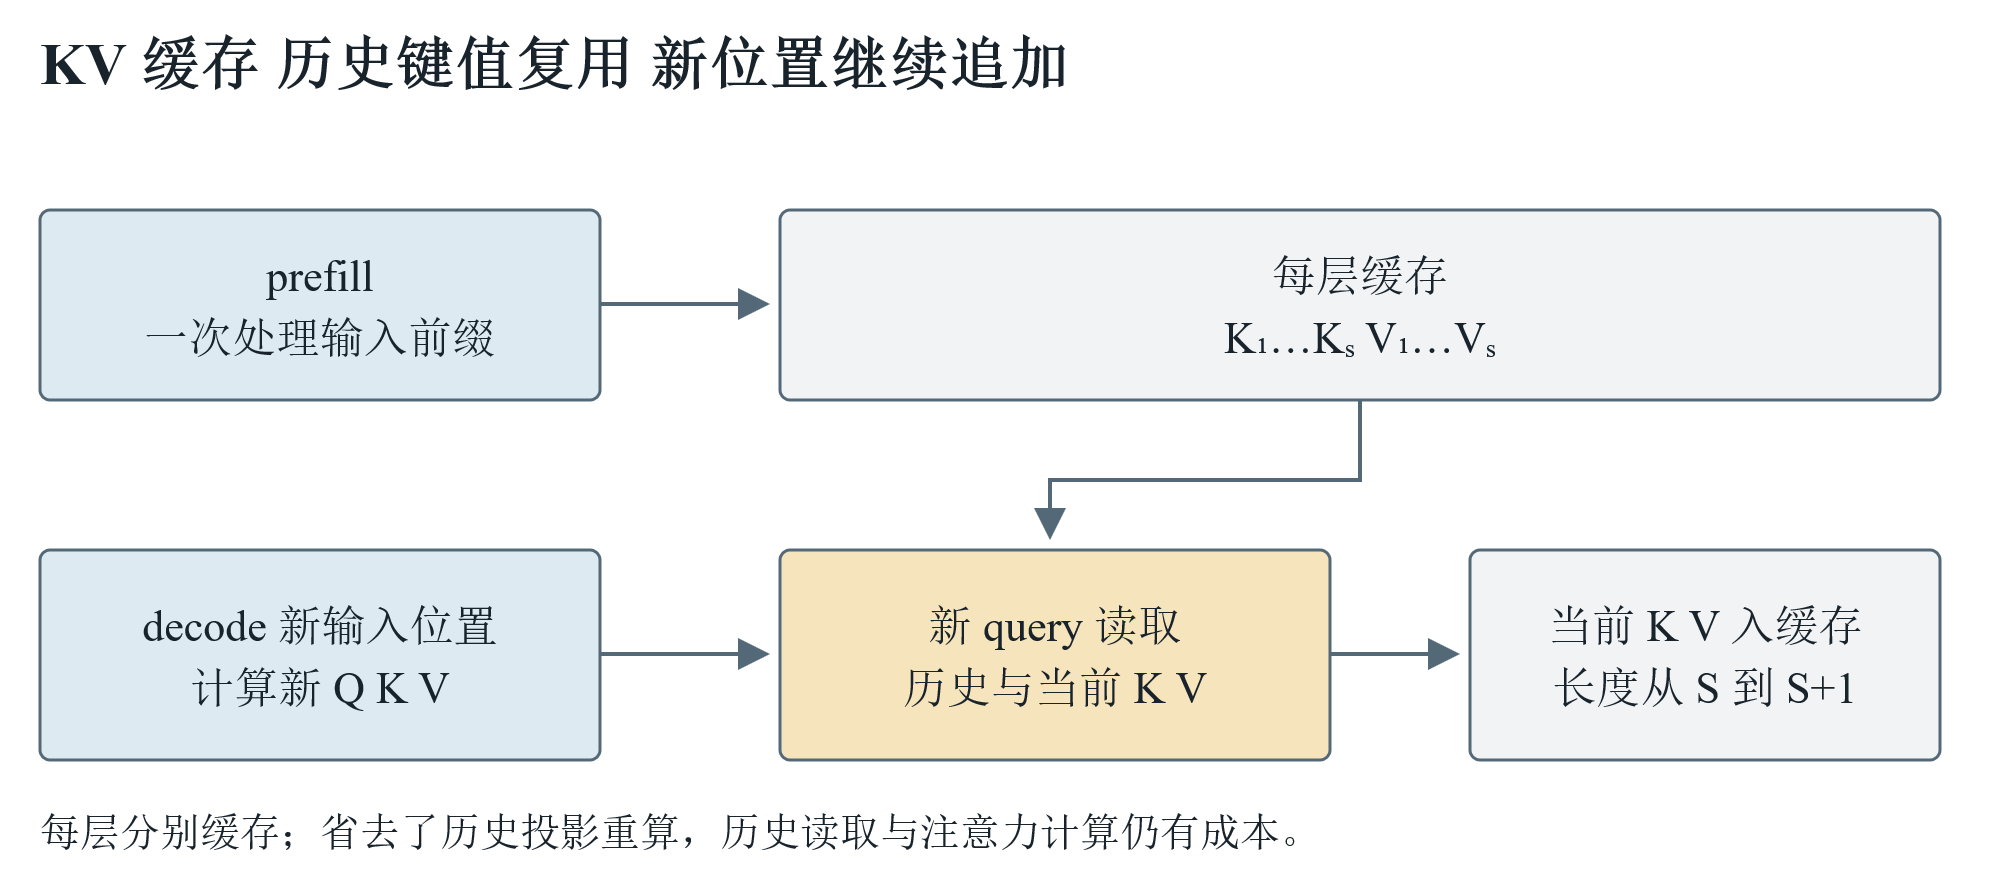
\includegraphics[width=\linewidth]{assets/media/image18.png}
    \caption{从 prefill 到 decode 的键值复用。每一层分别保存已处理位置的键和值；当前位置的查询读取这些缓存，计算注意力输出。}
    \label{fig:KV缓存复用}
\end{figure}

对一个简化的稠密注意力模型，单序列缓存占用可按两份张量、层数、KV 头数、头维度、序列长度与每元素字节数相乘估算。分组查询注意力（Grouped-Query Attention，GQA）让多个查询头共享一组 K、V，因此缓存容量由实际的 KV 头数决定。 用 M 表示字节占用，L 表示层数、H 的下标 KV 表示 KV 头数、d 表示头维度、S 表示缓存长度、b 表示每元素字节数，估算式为：
\[M_{KV} \approx 2\, L\, H_{KV}\, d\, S\, b\]

系数 2 对应 key 与 value 两份缓存。多个会话并发时，总缓存占用可以按各个会话的序列长度分别计算后求和。

例如 32 层、8 个 KV 头、每头 128 维、4096 个 token、每元素 2 字节，单序列 KV 约为 512 MiB。MiB 是二进制兆字节（mebibyte），1 MiB 等于 1,048,576 字节。完整的显存预算由模型权重、KV 缓存、计算临时缓冲和分配管理开销共同组成。缓存量化通过降低每元素字节数减少占用，滑动窗口通过限制保留的历史范围控制缓存长度。容量规划可以先按各会话长度估算 KV 缓存，再加上权重与运行时开销，确定可支持的并发规模。

FlashAttention 通过更好的计算与存储访问方式降低注意力的内存开销；PagedAttention 一类方案改善服务时的缓存管理。FlashAttention 侧重注意力计算中的数据读写与中间结果组织，PagedAttention 侧重多个请求的缓存分配与复用。评估服务性能时，首 token 延迟反映开始响应的等待时间，每秒生成 token 数反映输出速度，并发吞吐反映服务总处理能力，峰值显存决定运行容量。

部署还涉及权重量化、批处理和推测解码等方法。我们先了解它们各自在压缩权重、摊薄计算或减少主模型串行调用中的作用，再按实际瓶颈验证。量化后的评估包括关键任务准确率、对话模板兼容性、生成速度和显存占用，用来选择适合部署目标的精度与性能配置。

长推理轨迹会同时增加训练时的轨迹采样成本，以及服务时的解码步数、缓存长度与响应延迟。推理预算可以按任务难度分配：复杂任务保留更多求解步骤，简单任务尽早给出答案。模型选择、推理预算与服务配置共同决定任务质量、响应时间和单次请求成本。

\textbf{本节相关资料}
\begin{enumerate}
    \item Dao 等，2022，\href{https://arxiv.org/abs/2205.14135}{FlashAttention Fast and Memory-Efficient Exact Attention with IO-Awareness} 。阅读重点：计算复杂度与存储访问成本为什么要分别考虑。
    \item Ainslie 等，2023，\href{https://arxiv.org/abs/2305.13245}{GQA Training Generalized Multi-Query Transformer Models from Multi-Head Checkpoints} 。阅读重点：KV 头共享怎样影响缓存。
    \item Kwon 等，2023，\href{https://arxiv.org/abs/2309.06180}{Efficient Memory Management for Large Language Model Serving with PagedAttention} 。阅读重点：多请求场景下的缓存组织。
\end{enumerate}

\section{线性注意力 资源受限时怎样保留长程信息}\label{线性注意力}

上一节讨论的 KV 缓存保存历史位置的键和值。上下文越长，需要保存和读取的历史数据就越多。对于显存有限的设备、大量并发会话和持续生成的长任务，历史信息的存储与访问成为推理成本的重要来源。线性注意力（linear attention）通过改变历史信息的组织方式降低这部分开销，正成为资源受限条件下大模型架构的新兴研究与应用方向。

\textbf{从逐个读取历史到维护状态}~标准因果注意力在生成第 $t$ 个 token 时，让当前位置的查询与前 $t$ 个位置的键比较，再对相应的值加权求和。把长度为 $N$ 的整段序列处理完，需要计算的查询与键的配对数量按 $N^2$ 增长。线性注意力则把历史键值逐步汇总到一个状态中，新 token 到来时更新状态，再用当前查询读取状态。它像一份随阅读持续更新的工作笔记：已经读过的内容进入笔记，接下来的问题通过笔记取出相关信息。

以一种基础的核特征线性注意力为例，可以把因果计算写成：
\[
S_t=S_{t-1}+\varphi(k_t)v_t^{\mathsf T},\qquad
z_t=z_{t-1}+\varphi(k_t),\qquad
 o_t=\frac{S_t^{\mathsf T}\varphi(q_t)}{z_t^{\mathsf T}\varphi(q_t)}.
\]
这里，$t$ 是序列位置；$q_t$、$k_t$、$v_t$ 分别是该位置的查询、键和值列向量；$\varphi$ 是把查询和键映射为非负特征向量的函数。$S_t$ 是汇总到位置 $t$ 的键值状态矩阵，$z_t$ 是用于归一化的键特征累加向量，初始状态 $S_0$、$z_0$ 均为零。$\varphi(k_t)v_t^{\mathsf T}$ 是外积，把当前键与值的关联写入状态；上标 $\mathsf T$ 表示转置。$o_t$ 是读取状态后得到的输出向量，分母用于归一化，实际计算可加入一个很小的正数保持数值稳定。

当特征维度和值向量维度固定时，每次状态更新与读取的计算量不随历史长度增长，处理整段序列的注意力计算量便随 $N$ 线性增长；``线性''指的就是对序列长度的这种依赖关系。递推生成时，线性注意力层保存固定形状的状态，用状态更新替代不断追加历史键值。这个变化直接减少了长序列解码时的历史缓存与读取需求。

\textbf{从基础状态累加到现代混合架构}~状态相当于把历史压缩进有限容量的记忆。现代方法进一步学习哪些内容应保留、遗忘或改写，例如通过门控调节记忆保留比例，通过增量更新修正已有的键值关联。混合架构把线性注意力层与完整注意力层组合：线性层高效更新历史状态，完整注意力层按位置访问历史内容，层的配比决定了记忆方式与资源开销。

Kimi 等主流大模型团队已经把线性注意力用于实际模型架构。月之暗面在 2025 年发布的 Kimi Linear 采用 Kimi Delta Attention（KDA）与多头潜在注意力（Multi-Head Latent Attention，MLA）混合的设计，并公开了模型权重和推理实现。KDA 通过细粒度门控管理有限状态记忆，MLA 层保留完整注意力的信息访问方式。Kimi Linear 展示了线性注意力从基础算法进入大规模预训练与推理部署的实践路径。

资源受限场景推动这条路线继续发展：固定形状的状态降低长会话的缓存增长，门控与记忆更新提高状态的信息利用率，混合层设计协调精确检索与持续计算。对于需要处理长文档、维护多轮工具轨迹或同时服务大量用户的模型，历史信息怎样进入记忆、记忆怎样被读取，已经成为模型架构设计的核心问题。

\textbf{本节相关资料}
\begin{enumerate}
    \item Katharopoulos 等，2020，\href{https://arxiv.org/abs/2006.16236}{Transformers are RNNs: Fast Autoregressive Transformers with Linear Attention}。阅读重点：核特征形式怎样把注意力改写成可递推计算。
    \item Kimi Team 等，2025，\href{https://arxiv.org/abs/2510.26692}{Kimi Linear: An Expressive, Efficient Attention Architecture}。阅读重点：KDA 的状态更新与门控，以及 KDA、MLA 混合架构的资源效率。
\end{enumerate}
